\documentclass[a4paper,11pt]{ltjsarticle}
% 数式
\usepackage{amsmath,amsfonts}
\usepackage{bm}
% 画像
\usepackage{graphicx}
\usepackage{circuitikz}
\usepackage{amsmath,amssymb}
\usepackage{siunitx}
\usepackage{float}
\usepackage{tikz}
\usepackage{askmaps}
\usepackage{multirow}
\usepackage{bigstrut}
\usepackage{slashbox}
\usepackage{rotating}
\usepackage{listings}
% 数式
\usepackage{physics}
\usepackage{mathtools}
% 画像
\usepackage{subcaption}
% 表
\usepackage{makecell}
% その他
\usepackage{url}
\usepackage{ascmac}
\usepackage{cases}
\usepackage{here}
\usepackage{upgreek}
% 日本語対応
\usepackage{luatexja}
\usepackage{luatexja-fontspec}

\AtBeginDocument{\RenewCommandCopy\qty\SI}


\definecolor{commentgreen}{RGB}{0,200,0}
\definecolor{eminence}{RGB}{120,80,250}
\definecolor{weborange}{RGB}{255,165,0}
\definecolor{frenchplum}{RGB}{10,150,200}
\definecolor{commentgreen}{RGB}{0,200,0}
\definecolor{eminence}{RGB}{120,80,250}
\definecolor{weborange}{RGB}{255,165,0}
\definecolor{frenchplum}{RGB}{10,150,200}

\lstset{
        language = {C},
        basicstyle = \ttfamily\small,
        keywordstyle=\color{eminence}\ttfamily\bfseries,
        commentstyle=\color{commentgreen}\textit,
    identifierstyle=\color{black}\ttfamily,
        xleftmargin=.35in,
        frame=lines,
    showstringspaces=false,
        numbers=left,
        stepnumber = 1,
        breaklines=true,
        numberstyle = \ttfamily\normalsize,
    tabsize=4,  
        emph={int, int8_t, int16_t, int32_t, int64_t, uint8_t, uint16_t, uint32_t, uint64_t, char, double, float, unsigned, void, bool},
        emphstyle={\color{blue}}, 
        morekeywords={>, <, ., ;, +, -, *, /, !, =, ~},
        breakindent = 10pt, 
        framexleftmargin=10mm, 
        columns=fixed,
        basewidth=0.5em,
        }

% 特定のスタイル設定
\lstdefinestyle{customtxt}{
  basicstyle=\ttfamily\footnotesize,
  backgroundcolor=\color{lightgray},
  frame=single,
  breaklines=true,
  columns=fullflexible,
  showspaces=false,
  showstringspaces=false,
  showtabs=false,
  tabsize=4,
}

\newcommand{\fig}[4]{
    \begin{figure}[htbp]
      \centering
      \includegraphics[width=#4\columnwidth]{./image/#1}
      \caption{#2}
      \label{fig:#3}
    \end{figure}
  }
\begin{document}


\section{目的}
セレクター回路のリバースエンジニアリングをして、回路図を作成すいる。デコード回路の作成では真理値表の作成・論理式の作成、ブレッドボードへの配線を行った。
リバースエンジニアリングでは逆の工程をたどるため回路を調べて回路図を作成し、真理値表の作成を行う。
\section{原理}
今回はセレクタ回路のリバースエンジニアリングを行う。そこで、今回使用するものを以下に説明する。
\subsection{セレクタ回路}
セレクタ回路は複数の入力を持ち、出力する信号を選ぶことが出来る回路である。
今回使用するセレクタ基板は入力が $A = [A_2, A_1, A_0]$、$B = [B_2, B_1, B_0]$、$C = [C_2, C_1, C_0]$の3つの入力を持ち、$SW1$、$SW0$の2つのスイッチで選択することが出来る。
$SW1$、$SW0$の入力によって、$A$、$B$、$C$のどれかが出力される。また、
出力は$OUT = [OUT_2,OUT_1,OUT_0]$と$EN$の2つの信号を持つ。
$EN$は有効信号であり、セレクタ回路の先につながる3bitと7セグLEDをデコードする基板上で、$EN$が$1$の時にのみLEDに出力されるようになっている。
そのため$EN$が$0$になるときの$SW0$、$SW1$はどちらも$OFF$になっているときは$OUT$は何を出力してもLEDには表示されないので$*$と表記する。
\subsection{汎用ロジックIC}
汎用ロジックICは、論理回路を実装するためのICであり、型番によって搭載されている論理ゲートが異なる。
今回使用するICを表\ref{tab:IC}に示す。
\begin{table}[htbp]
  \centering
  \caption{IC}
  \begin{tabular}{|c|c|}
    \hline
    型番  &  機能  \\
    \hline
    74LS04 & NOTゲート \\
    74LS08 & ANDゲート \\
    74LS32 & ORゲート \\
    \hline
  \end{tabular}
  \label{tab:IC}
\end{table}
\subsection{動作確認用減算基盤}
今回使用するセレクタ回路の入力をするための基盤を動作確認用減算基盤という。
この基板はセレクタ回路とピンヘッダを介してつながっており、出力は$A= [A_2, A_1, A_0]$、$B = [B_2, B_1, B_0]$、$C = [C_2, C_1, C_0]$の3つの入力がある。
それぞれの出力に対して10進数から2進数にエンコードする回路が入っており、0から9までの入力をセレクタ回路に渡すことが可能であるが3bitの出力なので8以上の信号では4bit目が切り捨てされるため0から始まる。
動作確認用減算基盤のピンヘッダのピンアサインを表\ref{tab:pin}に示す。
\begin{table}[htbp]
  \centering
  \caption{ピンヘッダ}
  \label{tab:pin}
  \begin{tabular}{|c|c|}
    \hline
    $SW1$  & $SW2$  \\
    \hline
    $5V$ & $B2$ \\
    $A2$ & $B1$ \\
    $A1$ & $B0$ \\
    $A0$ & $C2$ \\
    $5V$ & $C1$ \\
    $5V$ & $C0$ \\
    $GND$ & $GND$ \\
    \hline
  \end{tabular}
\end{table}
\subsection{動作確認用デコード基板}
今回使用するセレクタ回路の出力を確認するための基板を動作確認用デコード基板という。
この基板はセレクタ回路とピンヘッダを介してつながっており、入力は$OUT = [OUT_2,OUT_1,OUT_0]$と$EN$の2つの信号がある。
\subsection{テスター}
テスターは交流・直流どちらでも使用できる電気計測器であり、電圧の測定や電流の測定、電圧を印加して抵抗値を調べるなどのことを行うことが出来る。
今回はテスターを用いることにより、どこのピンとどこのピンが導通しているかを確認する。
テスターを用いて回路をリバースエンジニアリングしていく。
\section{実験方法}
\subsection{セレクタ回路の動作確認}
まず最初にセレクタ基板にロ軸ICを挿入し、ピンヘッダを介して動作確認用減算基盤、動作確認用デコード基板を接続する。
セレクタ基板の概要図を図\ref{fig:selector}に示す。
$J1$に動作確認用減算基盤を接続し、$J2$に動作確認用デコード基板を接続する。
$IC1$から$IC6$に接続する汎用ロジックICを表\ref{tab:IC}に示す。
\fig{kiban.drawio.png}{セレクタ基板}{selector}{0.6}
\begin{table}[htbp]
  \centering
  \caption{IC}
  \begin{tabular}{|c|c|}
    \hline
    部品ID  &  汎用ロジックIC  \\
    \hline
    IC1  &  74LS04  \\
    IC2  &  74LS08  \\
    IC3  &  74LS08  \\
    IC4  &  74LS08  \\
    IC5  &  74LS32  \\
    IC6  &  74LS32  \\
    \hline
  \end{tabular}
\end{table}
\newpage
\subsection{リバースエンジニアリング}
リバースエンジニアリングを行っていく。このとき導通チェックのためにテスターの端子に電圧を印加させるため、ソケットからICを外して行う。
むやみにテスターを当てていくよりも、最も原始的なセレクタ回路を基にテスターを当てていくことである程度見るピンの数を減らすことが出来る。
最も原始的なセレクタ回路を図\ref{fig:selector}に示す。
\fig{selector.png}{最も原始的なセレクタ回路}{selector}{1}
\section{結果}
\subsection{セレクタ回路の動作確認}
セレクタ回路の動作確認を行った結果を表\ref{tab:selector}に示す。
3bitしか出力がないため、$(8)_10$以上の数値を入力しても4bit目が切り捨てられるため、$(8)_10$のときは 
\scalebox{0.023}{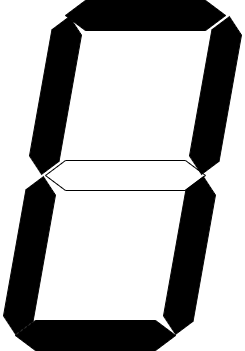
\includegraphics{./image/7segen.drawio.png}} が表示される。
\begin{table}[h]
  \centering
  \caption{セレクタ回路の動作確認}
  \begin{tabular}{|c|c|c|c|c|}
    \hline 
    \textrm{$(0)_{10}$} & \textrm{$(1)_{10}$} & \textrm{$(2)_{10}$} & \textrm{$(3)_{10}$} & \textrm{$(4)_{10}$} \\
    \hline
    \begin{minipage}{0.15\columnwidth}
      \centering
      \scalebox{0.15}{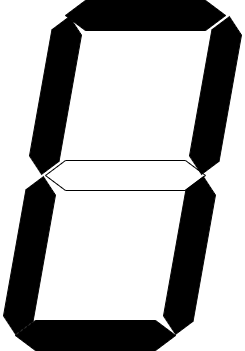
\includegraphics{./image/7seg0.drawio.png}}
    \end{minipage} &
    \begin{minipage}{0.15\columnwidth}
      \centering
      \scalebox{0.15}{
\includegraphics{./image/7seg1.drawio.png}}
    \end{minipage} &
    \begin{minipage}{0.15\columnwidth}
      \centering
      \scalebox{0.15}{
\includegraphics{./image/7seg2.drawio.png}}
    \end{minipage} &
    \begin{minipage}{0.15\columnwidth}
      \centering
      \scalebox{0.15}{
\includegraphics{./image/7seg3.drawio.png}}
    \end{minipage} &
    \begin{minipage}{0.15\columnwidth}
      \centering
      \scalebox{0.15}{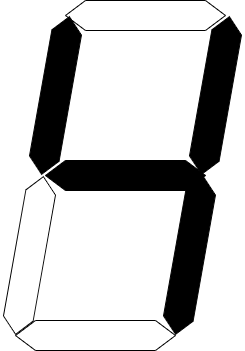
\includegraphics{./image/7seg4.drawio.png}}
    \end{minipage} \\
    \hline
    \textrm{$(5)_{10}$} & \textrm{$(6)_{10}$} & \textrm{$(7)_{10}$} & \textrm{$(8)_{10}$} & \textrm{$(9)_{10}$} \\
    \hline
    \begin{minipage}{0.15\columnwidth}
      \centering
      \scalebox{0.15}{
\includegraphics{./image/7seg5.drawio.png}}
    \end{minipage} &
    \begin{minipage}{0.15\columnwidth}
      \centering
      \scalebox{0.15}{
\includegraphics{./image/7seg6.drawio.png}}
    \end{minipage} &
    \begin{minipage}{0.15\columnwidth}
      \centering
      \scalebox{0.15}{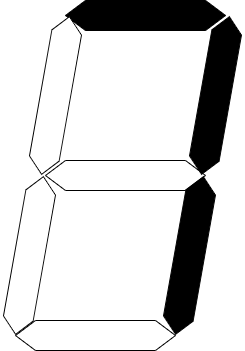
\includegraphics{./image/7seg7.drawio.png}}
    \end{minipage} &
    \begin{minipage}{0.15\columnwidth}
      \centering
      \scalebox{0.15}{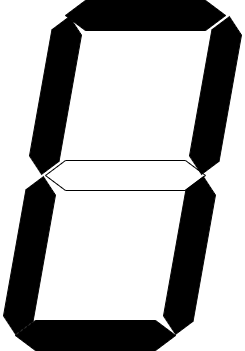
\includegraphics{./image/7segen.drawio.png}}
    \end{minipage} &
    \begin{minipage}{0.15\columnwidth}
      \centering
      \scalebox{0.15}{
\includegraphics{./image/7seg1.drawio.png}}
    \end{minipage} \\
    \hline
  \end{tabular} 
  \label{tab:selector}
\end{table}
\subsection{リバースエンジニアリング}
リバースエンジニアリングを行って作成した回路図を図\ref{fig:reverse}に示す。
\begin{figure}
  \centering
  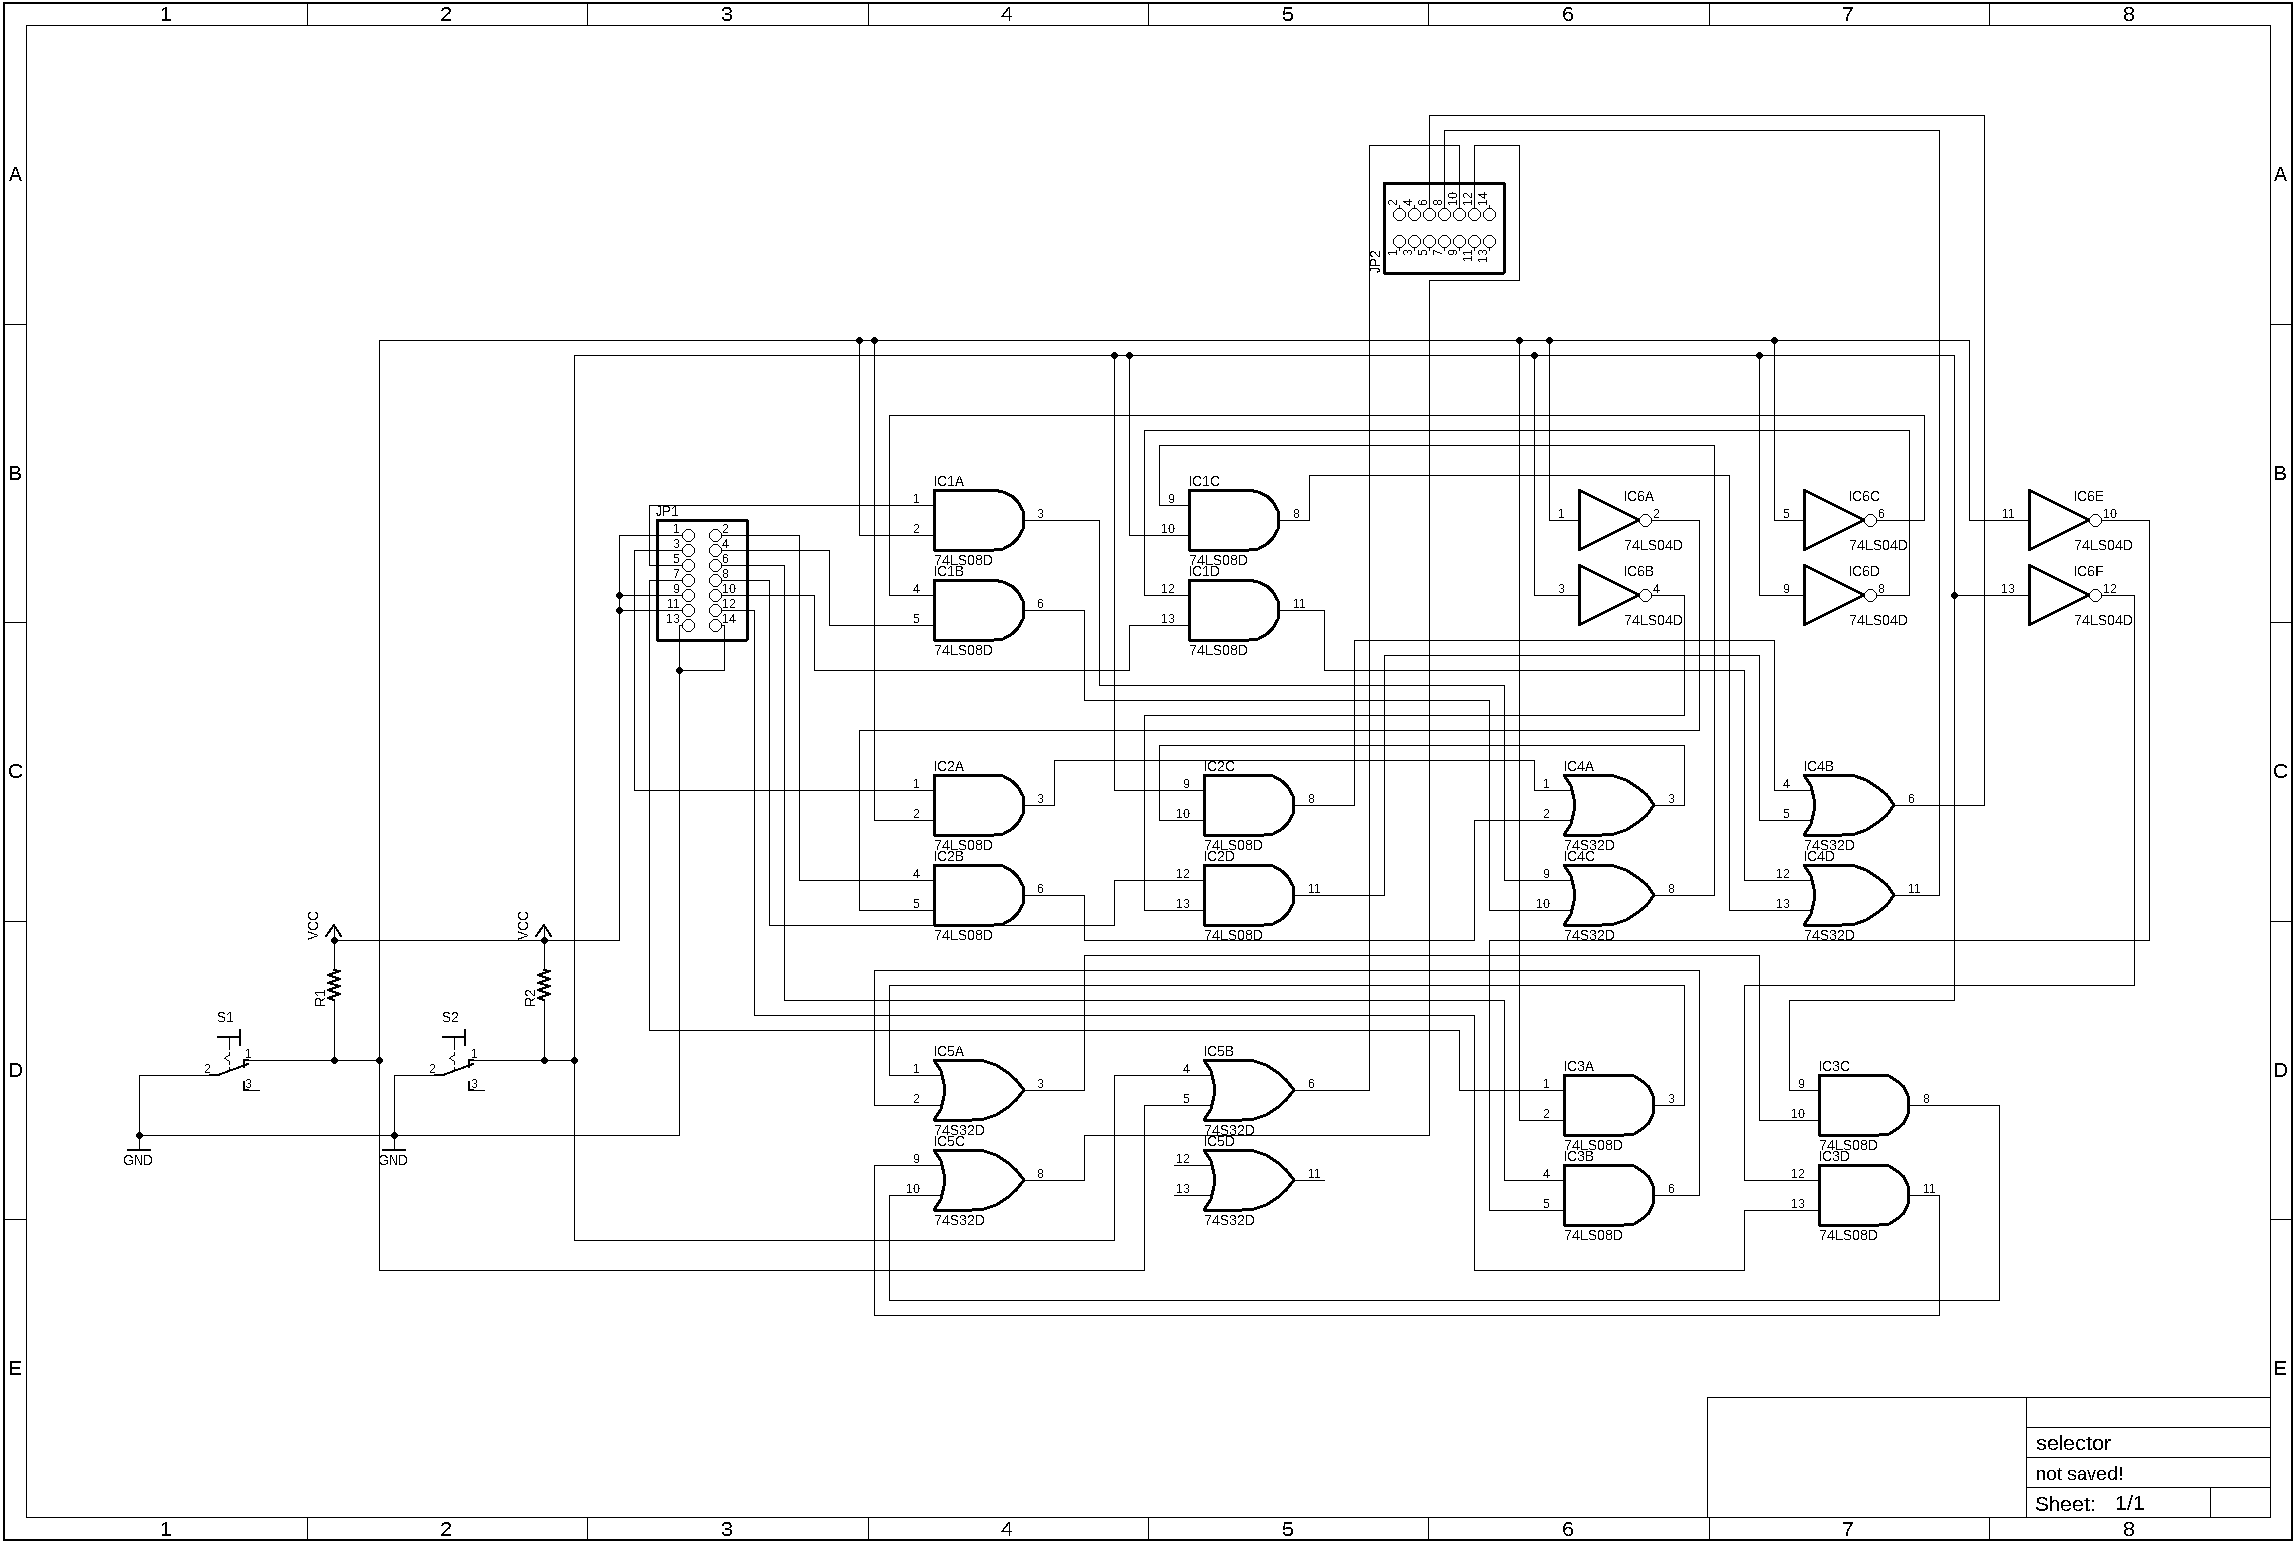
\includegraphics[angle = 90 , width =0.9\columnwidth]{./image/circuit.png}
  \caption{リバースエンジニアリングした回路図}
  \label{fig:reverse}
\end{figure}
\newpage
\section{考察}
セレクタ回路の予想をたてて、リバースエンジニアリングを行うことにより一個の入力当たり調べるピンの数が減り、
効率的に回路図を作成することが出来た。
\section{報告事項}
報告事項として報告するものを以下に示す。ただし、これは報告事項の原文を描いたものであるので図表の参照が行われていないものである。
この箇条書きの順番に報告事項$(a)$、報告事項$(b)$\dots として報告する。
\begin{itemize}
  \item 表$3.3$のように真理値表をまとめてください。
  \item 図$3.8$に示したトグルスイッチの接続方法について、どちらの接続方法が好ましいか、その理由を明確に報告してください。
  \item バイパスコンデンサについて調べてください。
  \item バイパスコンデンサの配置で適切なものは、$C1$と$C2$のいずれなのか、理由を加えて答えてください。
  \item 回路図を作成してください。このとき、抵抗やコンデンサなどの値もあわせて記入するようにしましょう。
\end{itemize}
\subsection{報告事項$(a)$}
表\ref{tab:a}に真理値表を示す。
\begin{table}[htbp]
  \centering
  \caption{真理値表}
  \begin{tabular}{|cc|cc|}
    \hline
    $SW1$  & $SW2$  &  $OUT$ & $EN$\\
    \hline
    0 & 0 &* & 0 \\
    0 & 1 &$B$ &1 \\
    1 & 0 &$C$ &1 \\
    1 & 1 &$A$ &1 \\
    \hline
  \end{tabular}
  \label{tab:a}
\end{table}
\subsection{報告事項$(b)$}
トグルスイッチでは、スイッチングする間に接点に接触していない時間存在する。そのため、接点が浮いている状態でもどちらかの入力が決まる接続方式が好ましい。
(a)の接続方法では、SW0の端子が常に抵抗を介して$+5V$と接続しており、スイッチが浮いている状態の時はSW0のほうに電流が流れる。接点が接触し、SW0とGNDが接続されるとSW0とGNDが同電圧になるため、SW0の出力は$0V$となる。
(b)の接続方法では、SW0の端子がスイッチングの間に浮いてしまうため、どっちつかずの状態になる。
これらのことから、(a)の接続方法が好ましい。
\subsection{報告事項$(c)$}
「デジタルICでは、処理する信号が「0」から「1」へ、または「1」から「0」に変化する際に、スイッチング電流とよばれる大きな電流が流れます。」\cite{参照ラベル名1}
このスイッチング電流はICの$V_{CC}$と$GND$の間に流れる。
スイッチング電流によりICの駆動に必要な電流が電源から供給できない場合には、ICの動作が不安定になることがある。
そのため、バイパスコンデンサを用いることで、足りない電流をコンデンサから供給することで、ICの駆動に必要な電流量を確保することが出来る。
\subsection{報告事項$(d)$}
バイパスコンデンサは電流が足りないときに賄うものであるが、電源の隣に配置してしまうとICが隣同士だった場合、手前のICにスイッチング電流が吸われて次のICが誤動作を引き起こすため
バイパスコンデンサを配置している意味がなくなってしまう。
そのため、ICとバイパスコンデンサを近づけて隣に配置することにより、安定してICを動作させることが出来る。
よって$C1$と$C2$のうち、$C2$が適切である。
\subsection{報告事項$(e)$}
作成した回路図を図\ref{fig:reverse}に示す。



\begin{thebibliography}{9}
  \bibitem{参照ラベル名1} 堀桂太郎、『デジタル回路入門早わかり(改定2版)』、株式会社オーム社、2016.7.13
\end{thebibliography}

\end{document}